\documentclass[a4paper,12pt]{report}
\usepackage[utf8]{inputenc}
\usepackage{newclude}
% This has include* command, necessary for including a file without creating a new page.
\usepackage{amsmath}
%http://ctan.org/pkg/amsmath
%Contains the 'implies' symbol, among other things.
%NOTES
% \(...\) is for inline math expressions.
% \[...\] is for properly indented math expressions.
\usepackage{hyperref}
%For enabling URL links and hypertext references in general.
\usepackage{fancyhdr}
%For making personalised header layouts.

\usepackage[breakable]{tcolorbox}
\usepackage{parskip} % Stop auto-indenting (to mimic markdown behaviour)

\usepackage{iftex}
\ifPDFTeX
    \usepackage[T1]{fontenc}
    \usepackage{mathpazo}
\else
    \usepackage{fontspec}
\fi

% Basic figure setup, for now with no caption control since it's done
% automatically by Pandoc (which extracts ![](path) syntax from Markdown).
\usepackage{graphicx}
% Maintain compatibility with old templates. Remove in nbconvert 6.0
\let\Oldincludegraphics\includegraphics
% Ensure that by default, figures have no caption (until we provide a
% proper Figure object with a Caption API and a way to capture that
% in the conversion process - todo).
\usepackage{caption}
\DeclareCaptionFormat{nocaption}{}
\captionsetup{format=nocaption,aboveskip=0pt,belowskip=0pt}

\usepackage{float}
\floatplacement{figure}{H} % forces figures to be placed at the correct location
\usepackage{xcolor} % Allow colors to be defined
\usepackage{enumerate} % Needed for markdown enumerations to work
\usepackage{geometry} % Used to adjust the document margins
\usepackage{amsmath} % Equations
\usepackage{amssymb} % Equations
\usepackage{textcomp} % defines textquotesingle
% Hack from http://tex.stackexchange.com/a/47451/13684:
\AtBeginDocument{%
    \def\PYZsq{\textquotesingle}% Upright quotes in Pygmentized code
}
\usepackage{upquote} % Upright quotes for verbatim code
\usepackage{eurosym} % defines \euro
\usepackage[mathletters]{ucs} % Extended unicode (utf-8) support
\usepackage{fancyvrb} % verbatim replacement that allows latex
\usepackage{grffile} % extends the file name processing of package graphics 
                        % to support a larger range
\makeatletter % fix for old versions of grffile with XeLaTeX
\@ifpackagelater{grffile}{2019/11/01}
{
    % Do nothing on new versions
}
{
    \def\Gread@@xetex#1{%
    \IfFileExists{"\Gin@base".bb}%
    {\Gread@eps{\Gin@base.bb}}%
    {\Gread@@xetex@aux#1}%
    }
}
\makeatother
\usepackage[Export]{adjustbox} % Used to constrain images to a maximum size
\adjustboxset{max size={0.9\linewidth}{0.9\paperheight}}

% The hyperref package gives us a pdf with properly built
% internal navigation ('pdf bookmarks' for the table of contents,
% internal cross-reference links, web links for URLs, etc.)
\usepackage{hyperref}
% The default LaTeX title has an obnoxious amount of whitespace. By default,
% titling removes some of it. It also provides customization options.
\usepackage{titling}
\usepackage{longtable} % longtable support required by pandoc >1.10
\usepackage{booktabs}  % table support for pandoc > 1.12.2
\usepackage[inline]{enumitem} % IRkernel/repr support (it uses the enumerate* environment)
\usepackage[normalem]{ulem} % ulem is needed to support strikethroughs (\sout)
                            % normalem makes italics be italics, not underlines
\usepackage{mathrsfs}

% Colors for the hyperref package
\definecolor{urlcolor}{rgb}{0,.145,.698}
\definecolor{linkcolor}{rgb}{.71,0.21,0.01}
\definecolor{citecolor}{rgb}{.12,.54,.11}

% ANSI colors
\definecolor{ansi-black}{HTML}{3E424D}
\definecolor{ansi-black-intense}{HTML}{282C36}
\definecolor{ansi-red}{HTML}{E75C58}
\definecolor{ansi-red-intense}{HTML}{B22B31}
\definecolor{ansi-green}{HTML}{00A250}
\definecolor{ansi-green-intense}{HTML}{007427}
\definecolor{ansi-yellow}{HTML}{DDB62B}
\definecolor{ansi-yellow-intense}{HTML}{B27D12}
\definecolor{ansi-blue}{HTML}{208FFB}
\definecolor{ansi-blue-intense}{HTML}{0065CA}
\definecolor{ansi-magenta}{HTML}{D160C4}
\definecolor{ansi-magenta-intense}{HTML}{A03196}
\definecolor{ansi-cyan}{HTML}{60C6C8}
\definecolor{ansi-cyan-intense}{HTML}{258F8F}
\definecolor{ansi-white}{HTML}{C5C1B4}
\definecolor{ansi-white-intense}{HTML}{A1A6B2}
\definecolor{ansi-default-inverse-fg}{HTML}{FFFFFF}
\definecolor{ansi-default-inverse-bg}{HTML}{000000}

% common color for the border for error outputs.
\definecolor{outerrorbackground}{HTML}{FFDFDF}

% commands and environments needed by pandoc snippets
% extracted from the output of `pandoc -s`
\providecommand{\tightlist}{%
    \setlength{\itemsep}{0pt}\setlength{\parskip}{0pt}}
\DefineVerbatimEnvironment{Highlighting}{Verbatim}{commandchars=\\\{\}}
% Add ',fontsize=\small' for more characters per line
\newenvironment{Shaded}{}{}
\newcommand{\KeywordTok}[1]{\textcolor[rgb]{0.00,0.44,0.13}{\textbf{{#1}}}}
\newcommand{\DataTypeTok}[1]{\textcolor[rgb]{0.56,0.13,0.00}{{#1}}}
\newcommand{\DecValTok}[1]{\textcolor[rgb]{0.25,0.63,0.44}{{#1}}}
\newcommand{\BaseNTok}[1]{\textcolor[rgb]{0.25,0.63,0.44}{{#1}}}
\newcommand{\FloatTok}[1]{\textcolor[rgb]{0.25,0.63,0.44}{{#1}}}
\newcommand{\CharTok}[1]{\textcolor[rgb]{0.25,0.44,0.63}{{#1}}}
\newcommand{\StringTok}[1]{\textcolor[rgb]{0.25,0.44,0.63}{{#1}}}
\newcommand{\CommentTok}[1]{\textcolor[rgb]{0.38,0.63,0.69}{\textit{{#1}}}}
\newcommand{\OtherTok}[1]{\textcolor[rgb]{0.00,0.44,0.13}{{#1}}}
\newcommand{\AlertTok}[1]{\textcolor[rgb]{1.00,0.00,0.00}{\textbf{{#1}}}}
\newcommand{\FunctionTok}[1]{\textcolor[rgb]{0.02,0.16,0.49}{{#1}}}
\newcommand{\RegionMarkerTok}[1]{{#1}}
\newcommand{\ErrorTok}[1]{\textcolor[rgb]{1.00,0.00,0.00}{\textbf{{#1}}}}
\newcommand{\NormalTok}[1]{{#1}}

% Additional commands for more recent versions of Pandoc
\newcommand{\ConstantTok}[1]{\textcolor[rgb]{0.53,0.00,0.00}{{#1}}}
\newcommand{\SpecialCharTok}[1]{\textcolor[rgb]{0.25,0.44,0.63}{{#1}}}
\newcommand{\VerbatimStringTok}[1]{\textcolor[rgb]{0.25,0.44,0.63}{{#1}}}
\newcommand{\SpecialStringTok}[1]{\textcolor[rgb]{0.73,0.40,0.53}{{#1}}}
\newcommand{\ImportTok}[1]{{#1}}
\newcommand{\DocumentationTok}[1]{\textcolor[rgb]{0.73,0.13,0.13}{\textit{{#1}}}}
\newcommand{\AnnotationTok}[1]{\textcolor[rgb]{0.38,0.63,0.69}{\textbf{\textit{{#1}}}}}
\newcommand{\CommentVarTok}[1]{\textcolor[rgb]{0.38,0.63,0.69}{\textbf{\textit{{#1}}}}}
\newcommand{\VariableTok}[1]{\textcolor[rgb]{0.10,0.09,0.49}{{#1}}}
\newcommand{\ControlFlowTok}[1]{\textcolor[rgb]{0.00,0.44,0.13}{\textbf{{#1}}}}
\newcommand{\OperatorTok}[1]{\textcolor[rgb]{0.40,0.40,0.40}{{#1}}}
\newcommand{\BuiltInTok}[1]{{#1}}
\newcommand{\ExtensionTok}[1]{{#1}}
\newcommand{\PreprocessorTok}[1]{\textcolor[rgb]{0.74,0.48,0.00}{{#1}}}
\newcommand{\AttributeTok}[1]{\textcolor[rgb]{0.49,0.56,0.16}{{#1}}}
\newcommand{\InformationTok}[1]{\textcolor[rgb]{0.38,0.63,0.69}{\textbf{\textit{{#1}}}}}
\newcommand{\WarningTok}[1]{\textcolor[rgb]{0.38,0.63,0.69}{\textbf{\textit{{#1}}}}}

% Define a nice break command that doesn't care if a line doesn't already exist.
\def\br{\hspace*{\fill} \\* }
% Math Jax compatibility definitions
\def\gt{>}
\def\lt{<}
\let\Oldtex\TeX
\let\Oldlatex\LaTeX
\renewcommand{\TeX}{\textrm{\Oldtex}}
\renewcommand{\LaTeX}{\textrm{\Oldlatex}}

% Pygments definitions
\makeatletter
\def\PY@reset{\let\PY@it=\relax \let\PY@bf=\relax%
\let\PY@ul=\relax \let\PY@tc=\relax%
\let\PY@bc=\relax \let\PY@ff=\relax}
\def\PY@tok#1{\csname PY@tok@#1\endcsname}
\def\PY@toks#1+{\ifx\relax#1\empty\else%
\PY@tok{#1}\expandafter\PY@toks\fi}
\def\PY@do#1{\PY@bc{\PY@tc{\PY@ul{%
\PY@it{\PY@bf{\PY@ff{#1}}}}}}}
\def\PY#1#2{\PY@reset\PY@toks#1+\relax+\PY@do{#2}}

\expandafter\def\csname PY@tok@w\endcsname{\def\PY@tc##1{\textcolor[rgb]{0.73,0.73,0.73}{##1}}}
\expandafter\def\csname PY@tok@c\endcsname{\let\PY@it=\textit\def\PY@tc##1{\textcolor[rgb]{0.25,0.50,0.50}{##1}}}
\expandafter\def\csname PY@tok@cp\endcsname{\def\PY@tc##1{\textcolor[rgb]{0.74,0.48,0.00}{##1}}}
\expandafter\def\csname PY@tok@k\endcsname{\let\PY@bf=\textbf\def\PY@tc##1{\textcolor[rgb]{0.00,0.50,0.00}{##1}}}
\expandafter\def\csname PY@tok@kp\endcsname{\def\PY@tc##1{\textcolor[rgb]{0.00,0.50,0.00}{##1}}}
\expandafter\def\csname PY@tok@kt\endcsname{\def\PY@tc##1{\textcolor[rgb]{0.69,0.00,0.25}{##1}}}
\expandafter\def\csname PY@tok@o\endcsname{\def\PY@tc##1{\textcolor[rgb]{0.40,0.40,0.40}{##1}}}
\expandafter\def\csname PY@tok@ow\endcsname{\let\PY@bf=\textbf\def\PY@tc##1{\textcolor[rgb]{0.67,0.13,1.00}{##1}}}
\expandafter\def\csname PY@tok@nb\endcsname{\def\PY@tc##1{\textcolor[rgb]{0.00,0.50,0.00}{##1}}}
\expandafter\def\csname PY@tok@nf\endcsname{\def\PY@tc##1{\textcolor[rgb]{0.00,0.00,1.00}{##1}}}
\expandafter\def\csname PY@tok@nc\endcsname{\let\PY@bf=\textbf\def\PY@tc##1{\textcolor[rgb]{0.00,0.00,1.00}{##1}}}
\expandafter\def\csname PY@tok@nn\endcsname{\let\PY@bf=\textbf\def\PY@tc##1{\textcolor[rgb]{0.00,0.00,1.00}{##1}}}
\expandafter\def\csname PY@tok@ne\endcsname{\let\PY@bf=\textbf\def\PY@tc##1{\textcolor[rgb]{0.82,0.25,0.23}{##1}}}
\expandafter\def\csname PY@tok@nv\endcsname{\def\PY@tc##1{\textcolor[rgb]{0.10,0.09,0.49}{##1}}}
\expandafter\def\csname PY@tok@no\endcsname{\def\PY@tc##1{\textcolor[rgb]{0.53,0.00,0.00}{##1}}}
\expandafter\def\csname PY@tok@nl\endcsname{\def\PY@tc##1{\textcolor[rgb]{0.63,0.63,0.00}{##1}}}
\expandafter\def\csname PY@tok@ni\endcsname{\let\PY@bf=\textbf\def\PY@tc##1{\textcolor[rgb]{0.60,0.60,0.60}{##1}}}
\expandafter\def\csname PY@tok@na\endcsname{\def\PY@tc##1{\textcolor[rgb]{0.49,0.56,0.16}{##1}}}
\expandafter\def\csname PY@tok@nt\endcsname{\let\PY@bf=\textbf\def\PY@tc##1{\textcolor[rgb]{0.00,0.50,0.00}{##1}}}
\expandafter\def\csname PY@tok@nd\endcsname{\def\PY@tc##1{\textcolor[rgb]{0.67,0.13,1.00}{##1}}}
\expandafter\def\csname PY@tok@s\endcsname{\def\PY@tc##1{\textcolor[rgb]{0.73,0.13,0.13}{##1}}}
\expandafter\def\csname PY@tok@sd\endcsname{\let\PY@it=\textit\def\PY@tc##1{\textcolor[rgb]{0.73,0.13,0.13}{##1}}}
\expandafter\def\csname PY@tok@si\endcsname{\let\PY@bf=\textbf\def\PY@tc##1{\textcolor[rgb]{0.73,0.40,0.53}{##1}}}
\expandafter\def\csname PY@tok@se\endcsname{\let\PY@bf=\textbf\def\PY@tc##1{\textcolor[rgb]{0.73,0.40,0.13}{##1}}}
\expandafter\def\csname PY@tok@sr\endcsname{\def\PY@tc##1{\textcolor[rgb]{0.73,0.40,0.53}{##1}}}
\expandafter\def\csname PY@tok@ss\endcsname{\def\PY@tc##1{\textcolor[rgb]{0.10,0.09,0.49}{##1}}}
\expandafter\def\csname PY@tok@sx\endcsname{\def\PY@tc##1{\textcolor[rgb]{0.00,0.50,0.00}{##1}}}
\expandafter\def\csname PY@tok@m\endcsname{\def\PY@tc##1{\textcolor[rgb]{0.40,0.40,0.40}{##1}}}
\expandafter\def\csname PY@tok@gh\endcsname{\let\PY@bf=\textbf\def\PY@tc##1{\textcolor[rgb]{0.00,0.00,0.50}{##1}}}
\expandafter\def\csname PY@tok@gu\endcsname{\let\PY@bf=\textbf\def\PY@tc##1{\textcolor[rgb]{0.50,0.00,0.50}{##1}}}
\expandafter\def\csname PY@tok@gd\endcsname{\def\PY@tc##1{\textcolor[rgb]{0.63,0.00,0.00}{##1}}}
\expandafter\def\csname PY@tok@gi\endcsname{\def\PY@tc##1{\textcolor[rgb]{0.00,0.63,0.00}{##1}}}
\expandafter\def\csname PY@tok@gr\endcsname{\def\PY@tc##1{\textcolor[rgb]{1.00,0.00,0.00}{##1}}}
\expandafter\def\csname PY@tok@ge\endcsname{\let\PY@it=\textit}
\expandafter\def\csname PY@tok@gs\endcsname{\let\PY@bf=\textbf}
\expandafter\def\csname PY@tok@gp\endcsname{\let\PY@bf=\textbf\def\PY@tc##1{\textcolor[rgb]{0.00,0.00,0.50}{##1}}}
\expandafter\def\csname PY@tok@go\endcsname{\def\PY@tc##1{\textcolor[rgb]{0.53,0.53,0.53}{##1}}}
\expandafter\def\csname PY@tok@gt\endcsname{\def\PY@tc##1{\textcolor[rgb]{0.00,0.27,0.87}{##1}}}
\expandafter\def\csname PY@tok@err\endcsname{\def\PY@bc##1{\setlength{\fboxsep}{0pt}\fcolorbox[rgb]{1.00,0.00,0.00}{1,1,1}{\strut ##1}}}
\expandafter\def\csname PY@tok@kc\endcsname{\let\PY@bf=\textbf\def\PY@tc##1{\textcolor[rgb]{0.00,0.50,0.00}{##1}}}
\expandafter\def\csname PY@tok@kd\endcsname{\let\PY@bf=\textbf\def\PY@tc##1{\textcolor[rgb]{0.00,0.50,0.00}{##1}}}
\expandafter\def\csname PY@tok@kn\endcsname{\let\PY@bf=\textbf\def\PY@tc##1{\textcolor[rgb]{0.00,0.50,0.00}{##1}}}
\expandafter\def\csname PY@tok@kr\endcsname{\let\PY@bf=\textbf\def\PY@tc##1{\textcolor[rgb]{0.00,0.50,0.00}{##1}}}
\expandafter\def\csname PY@tok@bp\endcsname{\def\PY@tc##1{\textcolor[rgb]{0.00,0.50,0.00}{##1}}}
\expandafter\def\csname PY@tok@fm\endcsname{\def\PY@tc##1{\textcolor[rgb]{0.00,0.00,1.00}{##1}}}
\expandafter\def\csname PY@tok@vc\endcsname{\def\PY@tc##1{\textcolor[rgb]{0.10,0.09,0.49}{##1}}}
\expandafter\def\csname PY@tok@vg\endcsname{\def\PY@tc##1{\textcolor[rgb]{0.10,0.09,0.49}{##1}}}
\expandafter\def\csname PY@tok@vi\endcsname{\def\PY@tc##1{\textcolor[rgb]{0.10,0.09,0.49}{##1}}}
\expandafter\def\csname PY@tok@vm\endcsname{\def\PY@tc##1{\textcolor[rgb]{0.10,0.09,0.49}{##1}}}
\expandafter\def\csname PY@tok@sa\endcsname{\def\PY@tc##1{\textcolor[rgb]{0.73,0.13,0.13}{##1}}}
\expandafter\def\csname PY@tok@sb\endcsname{\def\PY@tc##1{\textcolor[rgb]{0.73,0.13,0.13}{##1}}}
\expandafter\def\csname PY@tok@sc\endcsname{\def\PY@tc##1{\textcolor[rgb]{0.73,0.13,0.13}{##1}}}
\expandafter\def\csname PY@tok@dl\endcsname{\def\PY@tc##1{\textcolor[rgb]{0.73,0.13,0.13}{##1}}}
\expandafter\def\csname PY@tok@s2\endcsname{\def\PY@tc##1{\textcolor[rgb]{0.73,0.13,0.13}{##1}}}
\expandafter\def\csname PY@tok@sh\endcsname{\def\PY@tc##1{\textcolor[rgb]{0.73,0.13,0.13}{##1}}}
\expandafter\def\csname PY@tok@s1\endcsname{\def\PY@tc##1{\textcolor[rgb]{0.73,0.13,0.13}{##1}}}
\expandafter\def\csname PY@tok@mb\endcsname{\def\PY@tc##1{\textcolor[rgb]{0.40,0.40,0.40}{##1}}}
\expandafter\def\csname PY@tok@mf\endcsname{\def\PY@tc##1{\textcolor[rgb]{0.40,0.40,0.40}{##1}}}
\expandafter\def\csname PY@tok@mh\endcsname{\def\PY@tc##1{\textcolor[rgb]{0.40,0.40,0.40}{##1}}}
\expandafter\def\csname PY@tok@mi\endcsname{\def\PY@tc##1{\textcolor[rgb]{0.40,0.40,0.40}{##1}}}
\expandafter\def\csname PY@tok@il\endcsname{\def\PY@tc##1{\textcolor[rgb]{0.40,0.40,0.40}{##1}}}
\expandafter\def\csname PY@tok@mo\endcsname{\def\PY@tc##1{\textcolor[rgb]{0.40,0.40,0.40}{##1}}}
\expandafter\def\csname PY@tok@ch\endcsname{\let\PY@it=\textit\def\PY@tc##1{\textcolor[rgb]{0.25,0.50,0.50}{##1}}}
\expandafter\def\csname PY@tok@cm\endcsname{\let\PY@it=\textit\def\PY@tc##1{\textcolor[rgb]{0.25,0.50,0.50}{##1}}}
\expandafter\def\csname PY@tok@cpf\endcsname{\let\PY@it=\textit\def\PY@tc##1{\textcolor[rgb]{0.25,0.50,0.50}{##1}}}
\expandafter\def\csname PY@tok@c1\endcsname{\let\PY@it=\textit\def\PY@tc##1{\textcolor[rgb]{0.25,0.50,0.50}{##1}}}
\expandafter\def\csname PY@tok@cs\endcsname{\let\PY@it=\textit\def\PY@tc##1{\textcolor[rgb]{0.25,0.50,0.50}{##1}}}

\def\PYZbs{\char`\\}
\def\PYZus{\char`\_}
\def\PYZob{\char`\{}
\def\PYZcb{\char`\}}
\def\PYZca{\char`\^}
\def\PYZam{\char`\&}
\def\PYZlt{\char`\<}
\def\PYZgt{\char`\>}
\def\PYZsh{\char`\#}
\def\PYZpc{\char`\%}
\def\PYZdl{\char`\$}
\def\PYZhy{\char`\-}
\def\PYZsq{\char`\'}
\def\PYZdq{\char`\"}
\def\PYZti{\char`\~}
% for compatibility with earlier versions
\def\PYZat{@}
\def\PYZlb{[}
\def\PYZrb{]}
\makeatother


% For linebreaks inside Verbatim environment from package fancyvrb. 
\makeatletter
    \newbox\Wrappedcontinuationbox 
    \newbox\Wrappedvisiblespacebox 
    \newcommand*\Wrappedvisiblespace {\textcolor{red}{\textvisiblespace}} 
    \newcommand*\Wrappedcontinuationsymbol {\textcolor{red}{\llap{\tiny$\m@th\hookrightarrow$}}} 
    \newcommand*\Wrappedcontinuationindent {3ex } 
    \newcommand*\Wrappedafterbreak {\kern\Wrappedcontinuationindent\copy\Wrappedcontinuationbox} 
    % Take advantage of the already applied Pygments mark-up to insert 
    % potential linebreaks for TeX processing. 
    %        {, <, #, %, $, ' and ": go to next line. 
    %        _, }, ^, &, >, - and ~: stay at end of broken line. 
    % Use of \textquotesingle for straight quote. 
    \newcommand*\Wrappedbreaksatspecials {% 
        \def\PYGZus{\discretionary{\char`\_}{\Wrappedafterbreak}{\char`\_}}% 
        \def\PYGZob{\discretionary{}{\Wrappedafterbreak\char`\{}{\char`\{}}% 
        \def\PYGZcb{\discretionary{\char`\}}{\Wrappedafterbreak}{\char`\}}}% 
        \def\PYGZca{\discretionary{\char`\^}{\Wrappedafterbreak}{\char`\^}}% 
        \def\PYGZam{\discretionary{\char`\&}{\Wrappedafterbreak}{\char`\&}}% 
        \def\PYGZlt{\discretionary{}{\Wrappedafterbreak\char`\<}{\char`\<}}% 
        \def\PYGZgt{\discretionary{\char`\>}{\Wrappedafterbreak}{\char`\>}}% 
        \def\PYGZsh{\discretionary{}{\Wrappedafterbreak\char`\#}{\char`\#}}% 
        \def\PYGZpc{\discretionary{}{\Wrappedafterbreak\char`\%}{\char`\%}}% 
        \def\PYGZdl{\discretionary{}{\Wrappedafterbreak\char`\$}{\char`\$}}% 
        \def\PYGZhy{\discretionary{\char`\-}{\Wrappedafterbreak}{\char`\-}}% 
        \def\PYGZsq{\discretionary{}{\Wrappedafterbreak\textquotesingle}{\textquotesingle}}% 
        \def\PYGZdq{\discretionary{}{\Wrappedafterbreak\char`\"}{\char`\"}}% 
        \def\PYGZti{\discretionary{\char`\~}{\Wrappedafterbreak}{\char`\~}}% 
    } 
    % Some characters . , ; ? ! / are not pygmentized. 
    % This macro makes them "active" and they will insert potential linebreaks 
    \newcommand*\Wrappedbreaksatpunct {% 
        \lccode`\~`\.\lowercase{\def~}{\discretionary{\hbox{\char`\.}}{\Wrappedafterbreak}{\hbox{\char`\.}}}% 
        \lccode`\~`\,\lowercase{\def~}{\discretionary{\hbox{\char`\,}}{\Wrappedafterbreak}{\hbox{\char`\,}}}% 
        \lccode`\~`\;\lowercase{\def~}{\discretionary{\hbox{\char`\;}}{\Wrappedafterbreak}{\hbox{\char`\;}}}% 
        \lccode`\~`\:\lowercase{\def~}{\discretionary{\hbox{\char`\:}}{\Wrappedafterbreak}{\hbox{\char`\:}}}% 
        \lccode`\~`\?\lowercase{\def~}{\discretionary{\hbox{\char`\?}}{\Wrappedafterbreak}{\hbox{\char`\?}}}% 
        \lccode`\~`\!\lowercase{\def~}{\discretionary{\hbox{\char`\!}}{\Wrappedafterbreak}{\hbox{\char`\!}}}% 
        \lccode`\~`\/\lowercase{\def~}{\discretionary{\hbox{\char`\/}}{\Wrappedafterbreak}{\hbox{\char`\/}}}% 
        \catcode`\.\active
        \catcode`\,\active 
        \catcode`\;\active
        \catcode`\:\active
        \catcode`\?\active
        \catcode`\!\active
        \catcode`\/\active 
        \lccode`\~`\~ 	
    }
\makeatother

\let\OriginalVerbatim=\Verbatim
\makeatletter
\renewcommand{\Verbatim}[1][1]{%
    %\parskip\z@skip
    \sbox\Wrappedcontinuationbox {\Wrappedcontinuationsymbol}%
    \sbox\Wrappedvisiblespacebox {\FV@SetupFont\Wrappedvisiblespace}%
    \def\FancyVerbFormatLine ##1{\hsize\linewidth
        \vtop{\raggedright\hyphenpenalty\z@\exhyphenpenalty\z@
            \doublehyphendemerits\z@\finalhyphendemerits\z@
            \strut ##1\strut}%
    }%
    % If the linebreak is at a space, the latter will be displayed as visible
    % space at end of first line, and a continuation symbol starts next line.
    % Stretch/shrink are however usually zero for typewriter font.
    \def\FV@Space {%
        \nobreak\hskip\z@ plus\fontdimen3\font minus\fontdimen4\font
        \discretionary{\copy\Wrappedvisiblespacebox}{\Wrappedafterbreak}
        {\kern\fontdimen2\font}%
    }%
    
    % Allow breaks at special characters using \PYG... macros.
    \Wrappedbreaksatspecials
    % Breaks at punctuation characters . , ; ? ! and / need catcode=\active 	
    \OriginalVerbatim[#1,codes*=\Wrappedbreaksatpunct]%
}
\makeatother

% Exact colors from NB
\definecolor{incolor}{HTML}{303F9F}
\definecolor{outcolor}{HTML}{D84315}
\definecolor{cellborder}{HTML}{CFCFCF}
\definecolor{cellbackground}{HTML}{F7F7F7}

% prompt
\makeatletter
\newcommand{\boxspacing}{\kern\kvtcb@left@rule\kern\kvtcb@boxsep}
\makeatother
\newcommand{\prompt}[4]{
    {\ttfamily\llap{{\color{#2}[#3]:\hspace{3pt}#4}}\vspace{-\baselineskip}}
}

% Prevent overflowing lines due to hard-to-break entities
\sloppy 
% Setup hyperref package
\hypersetup{
    breaklinks=true,  % so long urls are correctly broken across lines
    colorlinks=true,
    urlcolor=urlcolor,
    linkcolor=linkcolor,
    citecolor=citecolor,
    }
% Slightly bigger margins than the latex defaults

\geometry{verbose,tmargin=1in,bmargin=1in,lmargin=1in,rmargin=1in}

\pagestyle{fancy}
\fancyhf{}
\rhead{Pranav Gopalkrishna, 1940223}

\title{Applications of Number Theory}
\author{Pranav Gopalkrishna, 1940223}

\begin{document}
\maketitle

\chapter{Pseudorandom numbers}
\section{Random numbers}
A random number is a measurement taken from a random i.e. non-deterministic process. i.e. a process whose future behaviour cannot be predicted with certainty. Hence, in general, a sequence of random numbers cannot be expressed as a generalised formula. Instead, a sequence of random numbers is defined using a probability distribution that associates possible value (that can be drawn from the process) to its probability of occurrence (i.e. the probability that the value occurs at any given point in time in the random process).
\\~\\
A sequence of numbers is said to be random if
\begin{itemize}
	\item Each number has equal probability of occurrence (uniformity)
	\item Any past value has no effect in determining the current value (independence)
\end{itemize}

\section{Pseudorandom numbers}
In theory, due to causality, a truly random process may not exist. In practice, randomness is determined by unpredictability from a realistic perspective, where there are constraints on time \& computational capacity. Hence, if a sequence possesses a sufficiently complicated pattern (often involving too many unaccountable factors) such that this pattern cannot or will not be realistically determined in a given situation, it may be considered random.
\\~\\
Computation is a deterministic process, hence its results are predictable, fundamentally. However, at a sufficient complexity, a computational process \& its results can be practically unpredictable for the given purposes.

\section{Pseudorandom number generation (pRNG)}
pRNG involves one arbitrary input, known as the seed. The seed is the starting point of the pRNG, \& may be the starting point of the sequence itself. A computational (mathematical) algorithm is applied in the seed to generate the pseudorandom sequence one number at a time. This process is usually recursive (i.e. using the previously generated number as an input to generate the next number), but it may simply a function of the seed, which is not preferred, since such a pattern is usually easier to crack.
\\~\\
1.\\
A sequence generated using a given seed for a given algorithm can be reproduced using the same seed for the same algorithm. Hence, the level of randomness of the pseudorandom sequence is dependent on the initial seed.
\\~\\
2.\\
A pseudorandom sequence containing values with a fixed maximum number of digits must eventually repeat, since the number of possible values that an occur in the sequence is finite, \& eventually, a previously used seed will be encountered \& reused (leading to a previously produced sequence of values). The length of the longest repeated sequence in a pRNG is called the period of the pRNG. Note that this repeated sequence may be not include the seed \& some or many of the previously generated pseudorandom numbers.
\\~\\
The above points 1 \& 2 clearly show that pseudorandom numbers are deterministic, fundamentally. However, this deterministic quality combined with the simulated randomness has many useful applications, which may not only rely on the practical unpredictability of the pRNG, but may also rely on the reproducibility of a pseudorandom sequence.

\section{Some applications of pRNG}
\subsection{Video game encounters}
In many video games, such as Minecraft, a player's experience is randomised to some degree, using pRNG. For example, it may be used to randomise the behaviour of certain NPCs (non-playable characters), the loot obtained in certain treasure chests, the drops obtained by mining a resource, etc. This often makes the game more engaging, since the player's experience is not entirely predictable, \& he or she is compelled to adapt \& improvise to varying degrees. Furthermore, since the pRNG is reproducible, the game can be designed in a way that the current game world produces the same outcomes for given actions or encounters for the player, if the player were to try to reload the game or go to a previous checkpoint.

\subsection{End-to-end encryption}
End-to-end encryption is a method to ensure that data shared between two users' devices cannot be intercepted \& accessed by a third-party. This involves the following steps:
\begin{itemize}
	\item Obtaining a common seed for pRNG, for the two devices only
	\item Generating a new secret key using pRNG to encrypt the new message,\\
	(Since the sender's \& receiver's pRNG start from the same seed, they obtain the same secret key)
	\item Generating the same secret key using pRNG to decrypt the new message
	\item Deleting the secret keys from in device
\end{itemize}
This involves generating a secret key for each message in the sender's \& receiver's separately.

\section{Some simple pseudrandom generators}
\include*{codes/tex/pRNG}

\chapter{Hashing function}
\section{Definition \& associated terms}
A hashing function is a function that maps given data of arbitrary size to a single value that has fixed size limit. Applying a hashing function on data is called "hashing the data". The return value of a hash function is called a hash value. In some implementations, the hash value is of fixed length.
\\~\\
Since hashing often involves converting any input into a hash value of limited (often smaller) size, hash functions may be called "compression functions". For a similar reason, a hash value is also called a message digest.

\section{Properties of an ideal hash function}
\subsection{Non-invertibility}
It should be computationally difficult to find the inverse of a hash function, i.e. given a hash value, the corresponding input must be difficult to compute. In other terms, if $h$ is the hash function, $h(x)=z$, \& only $z$ is known, $x$ must be difficult to compute.

\subsection{Collision resistance i.e. one-to-one property}
The mapping of two or more inputs to the same hash value i.e. collisions must be rare, \& ideally impossible. In other terms, it must be difficult to find two inputs $x$ \& $y$ such that $h(x)=h(y)=z$. However, since inputs are of arbitrary length while hash values are of limited length, collisions are impossible to eliminate entirely.

\subsection{Second pre-image resistance}
This is related to collision resistance, but here we specify that \textit{given an input \& hash value pair}, it should be computationally difficult to find another input that has the same hash value. In other terms, given a hash value $z$ for a pre-image $x$ i.e. for $h(x)=z$, it must be difficult to obtain another pre-image $y \neq x$ such that $h(y)=z$. Note that collision resistance implies second pre-image resistance.

\section{Design \& implementation}
At the most basic level, a hash function can simply operate on an input to produce an output that has a fixed size limit. Now, note that hash functions are often used for creating hash tables (also called hash maps). Hash tables are arrays that can associate a key to a value. Hence, we can use the hash value of a given input to perform a direct lookup in the table, to see
\begin{itemize}
	\item Whether the given input is a key that exists for the hash map
	\item What values correspond to the given key
\end{itemize}

For this purpose, the hash value must be a sufficiently small integer that can serve as an index in the hash table. With this in mind, we will follow two steps in the creation of the hash function:
\begin{itemize}
	\item Map a key to an integer
	\item Map the integer to a bucket i.e. a sufficiently small positive integer
\end{itemize}

\subsection{Sample code}
\include*{codes/tex/hashFunctions}

\chapter{Parity bit method}
\section{Context}
Digital data is stored, processed \& transmitted as binary information i.e. information encoded using only two units, conventionally represented as 0 \& 1. Our concern is with data transmission. Due to factors such as noise or distortion, the data sent may not match the data received. In binary data, this means that certain 0's may become 1 or certain 1's may become 0. The deviation between the sent data \& received data is the error. We have multiple methods error detection, \& parity bit method is one of them.

\section{Definition}
Parity bit method is a method to detect single bit errors i.e. when the sent data \& received data differ by only one bit (this method may fail for multiple bit errors). In this method, the receiver checks whether the number of 1's in the received data is even or odd. For even parity check, the data is considered correct only if the number of 1's is even, \& correspondingly for odd parity check. To enable such a parity check, the sender appends a parity bit to the data it sends. For even parity check, the sender sets the parity bit such that the number of 1's including the parity bit is even, \& correspondingly for odd parity check.
\\~\\
In other terms, the parity bit can be defined as $n \bmod 2$, where $n$ is the sum of the binary digits of the message (hence, $n$ is the number of 1's in the message).

\section{Basic parity bit method}
Here, a parity bit is simply appended after the data bit sequence, based on the number of ones in the binary data i.e. the sum of the binary digits.

\subsection{Implementation}
\include*{codes/tex/parityBitMethodBasics}

\section{Hamming code}
Hamming code is the utilisation of parity bits to make the error detection more precise \& even enable some error correction. The idea of Hamming code is that instead of using one parity bit for the whole data, we use multiple parity bits that help detect errors in different sections of the data. The algorithm of Hamming code is as follows...

\begin{itemize}
	\item Obtain the bit positions starting from 1 in binary form\\(1, 10, 11, 100...)
	\item Bit positions that are powers of 2 are marked as parity bits\\(1, 2, 4, 8...)
	\item Other bit positions are marked as data bits
\end{itemize}

Each parity bit is meant for the following sequences...

\begin{itemize}
	\item Parity bit 1 covers all the bits positions whose binary representation has 1 in the least significant position\\(1, 3, 5...)
	\item Parity bit 2 covers all the bits positions whose binary representation has 1 in the 2nd position from the least significant bit\\(2, 3, 6...)
	\item Parity bit 4 covers all the bits positions whose binary representation has 1 in the 3rd position from the least significant bit\\(4, 5, 6...)
	\item Parity bit 8 covers all the bits positions whose binary representation has 1 in the 4th position from the least significant bit bits\\(8, 9, 10...)
\end{itemize}

In general, each parity bit covers all bits where the bitwise \& of the parity position \& the bit position is non-zero. Keep adding parity bits as long as the last parity bit position is before at least one data bit. Note that parity bits are omitted from the count of 1's, so whenever they are encountered, just ignore \& move on.

\subsection{Some results}
Define the following:

\begin{itemize}
	\item $r$ is the number of parity bits required for a data sequence
	\item $m$ is the number of data bits
\end{itemize}

Now, notice that

\begin{itemize}
	\item Parity bit 1 is in position $1=2^0$
	\item Parity bit 2 is in position $2=2^1$
	\item Parity bit 3 is in position $4=2^2$
	\item Parity bit 4 is in position $8=2^3$
\end{itemize}

Hence, in general, parity bit $k$ is in the position $2^{k-1}$. Hence, the last parity bit i.e. parity bit $r$ is in the position $2^{r-1}$. The fact that this is the last parity bit means that $2^{r-1}$ is the last power of 2 that is less than the size of the whole message (message includes the data bits \& parity bits). Hence, $2^r$ is the first power of 2 that is greater than the size of the whole message. Now, note that the size of the message is given by $m+r$. Hence,
\[2^r > m+r\]
\begin{equation}\implies 2^r \geq m+r+1\end{equation}

We will use this result to insert the right amount of redundant i.e. parity bits to the sequence of data bits as we create the whole message.

\subsection{Implementation}
\include*{codes/tex/parityBitMethodusingHammingCode}

\chapter{Cryptography}
\section{Definition \& associated terms}
Cryptography is the study \& practice of secure communication techniques wherein the message's contents can only be viewed by the sender(s) \& intended receiver(s) (\textit{"kryptos" $\implies$ hidden (Greek)}). An interceptor is an unauthorised entity who can access the transmitted data (but may not be able to read the message itself).

\subsection{Cryptosystem \& its components}
A cryptosystem (also called cipher system) is an implementation of cryptographic techniques, \& involves the accompanying infrastructure. A basic cryptosystem has the following components:

\begin{itemize}
	\item Plaintext
	\item Encryption key
	\item Encryption algorithm
	\item Ciphertext
	\item Decryption algorithm
	\item Decryption key
\end{itemize}

Plaintext is the data to be messaged. Encryption key is a value known by the sender. Encryption algorithm is a computational process whose inputs are the plaintext \& the encryption key, \& whose output is the ciphertext, which is a transformed version of the plaintext (\textit{note that the ciphertext may be accessed by any interceptor who has access to the communication channel}). Decryption algorithm is a computational process whose inputs are the ciphertext \& the decryption key, \& whose intended output is the plaintext. Decryption key is a value known by the receiver, \& related to the encryption key such that when it is applied to the decryption algorithm, it transforms the ciphertext back to the plaintext.

\subsection{Cryptography classification}
Cryptography can be classified into the following categories:
\begin{itemize}
	\item Symmetric cryptography
	\item Asymmetric cryptography
	\item Hashing (discussed separately)
\end{itemize}
\\~\\
\textbf{\underline{NOTE 1}: Symmetric vs. asymmetric key cryptography}\\
In symmetric cryptography, the decryption key \& encryption key are identical. In asymmetric cryptography, they differ, but are still related to each other, since the decryption key must be made with respect to the encryption key to enable decryption, because that the encryption key plays a major role in shaping the ciphertext.
\\~\\
\textbf{\underline{NOTE 2}: Key space}\\
In asymmetric cryptography, there can be multiple decryption keys provided to different receivers. The set of all possible decryption keys that can be provided for a given cryptosystem is called the key space of the cryptosystem. This becomes relevant when we discuss public keys.

\section{Private \& public keys}
\subsection{Private keys \& symmetric cryptography}
A private key is a key used in symmetric cryptography, hence is used for both encryption \& decryption. It is private i.e. known only to the sender \& receiver, \& kept secret. For example, the end-to-end encryption (discussed in the pseudorandom numbers chapter) in a messaging service such as WhatsApp uses private keys that are known only by the two or more parties of a chat. \textit{Note that in this example, the private keys change for every message, based on a pseudorandom sequence generated separately by each device registered in the chat.}

\subsection{Public keys \& asymmetric cryptography}
A public key is an encryption key that is publicly visible in a network, \& is associated with a particular member of the network. This public key is used to encrypt messages intended for the particular member, who then uses a different private decryption key to decrypt the message. Since the encryption \& decryption keys differ, this is asymmetric cryptography.
\\~\\
To understand public keys, consider the following situation. Let's say we own a network with multiple people connected to it. To make our network secure i.e. resistant to interception of messages, we want to use encryption \& decryption to ensure that only the intended receiver can read the message. However, we also have the following desires for the network:

\begin{itemize}
	\item Anyone can communicate with anyone else in the network
	\item A new member can be easily added to the network
	\item Establishing a secure communication must be automatic \& seamless
\end{itemize}

If we were to use private keys, then everyone would need to know everyone else's private keys, \& hence, the network would not be secure. Hence, we create a system wherein:

\begin{itemize}
	\item Every device has its own public encryption key visible to other members
	\item A message is encrypted using the public key of the intended receiver
	\item A message is decrypted locally using a different private decryption key
\end{itemize}

A member's public encryption key must be such that a message encrypted using this key can only be decrypted by this member's own decryption key. Furthermore, since the decryption keys are private \& different from the public keys, no one should be able to read messages intended for someone else, since they do not have the required decryption key.

\section{Rivest-Shamir-Adleman algorithm}
RSA is a public key cryptosystem that is widely used today to ensure secure digital communications. The basic idea behind it is as follows...
\\~\\
Let $m$ be a given positive integer, \& let $e$, $d$ \& $n$ (where $n>m$) be large positive integers that satisfy the congruence $(m^e)^d \equiv m \pmod n$ (i.e. the remainder of $(m^e)^d/n$ is the same as the remainder of $m/n$). If  $e$ \& $n$ are large numbers, it can be extremely difficult to deduce  $d$for a given  $m$, even if $e$, $m$ \& $n$ are known. This is the basis of RSA algorithm. In this algorithm, we have

\begin{itemize}
	\item $p$ \& $q$ are two distinct large primes (which are kept secret)
	\item $m$ as the reversible integer of the original message constructed in a way such that $m$ is divisible by neither $p$ nor $q$ (reversible $\implies$ original string can be reliably obtained)
	\item $n$ (where $n>m$) is the product of $p$ \& $q$
	\item $(n, e)$ is the public encryption key
	\item  $(n, d)$ is the private decryption key
\end{itemize}

The RSA algorithm is constructed in such a manner that the message encrypted for an intended receiver (using that receiver's public encryption key) can be decrypted in a reasonable amount of time only if the receiver's private decryption key is used.

\subsection{Obtaining the public \& private keys}
\textbf{(i.e. constructing $e$ \& $d$ such that $(m^e)^d \equiv m \pmod n$)}
\subsubsection{Introduction to the problem}
By Fermat's little theorem, we have that for any prime $p$ \& any positive integer $m$ that is not divisible by $p$, $m^{p-1} \equiv 1 \pmod p \implies m^p \equiv m \pmod p$. Now, note that we from this, we can derive a result that states that for any two primes $p$ \& $q$, $m^{pq} \equiv m \pmod {pq}$, from which we can get $e=p, d=q$ or $e=q, d=p$. But this is obviously not secure, since if any one prime is known, the other can be easily deduced by dividing $n$ \textif{(hence, since public encryption key is visible to everyone, decryption key can be easily found for any potential receiver)}. Hence, we use another approach...

\subsubsection{Using the Carmichael function}
The Carmichael function of any positive integer $x$ (denoted by $\lambda(x)$) is the smallest positive (hence non-zero) integer $k$ such that $a^k \equiv 1 \pmod x$ for any positive integer $a<x$ that is coprime to x.  Note the following results for Carmichael function:

\begin{itemize}
	\item If $x$ is prime, $\lambda(x)=x-1$
	\item If $x=p_1^{k_1}p_2^{k_2}...p_r^{k_r}$ (where $\{p_i\}$ are distinct primes),\\$\lambda(x)=lcm(\lambda(p_1^{k_1}),\lambda(p_2^{k_2}...\lambda(p_r^{k_r}))$
\end{itemize}
\\~\\
We will use this function \& the above results to obtain a suitable $e$.
Consider...

\begin{itemize}
	\item $p$ \& $q$ are primes, hence $\lambda(p)=p-1$ \& $\lambda(q)=q-1$
	\item $p \nmid m \implies m^{p-1} \equiv 1 \pmod p$ (by Fermat's little theorem)
	\item $q \nmid m \implies m^{q-1}  \equiv 1 \pmod q$ (by Fermat's little theorem)
	\item From the above, we get $m^{\lambda(p)} \equiv 1 \pmod p$ \& $m^{\lambda(q)} \equiv 1 \pmod q$
	\item $n=pq \implies \lambda(n) = \lambda(pq) = lcm(\lambda(p), \lambda(q))$
\end{itemize}
\\~\\
Now consider $m^{\lambda(p)} \equiv 1 \pmod p$ alone...
\[m^{\lambda(p)} \equiv 1 \pmod p\]
\[\implies (m^{\lambda(p)})^k \equiv 1^k \pmod p\]
\begin{equation} \label{eq1} \implies m^{k\lambda(p)} \equiv 1 \pmod p\end{equation}
Also, we have the trivial congruence
\begin{equation} \label{eq2} m \equiv m \pmod p\end{equation}
Hence, we get
\begin{equation} \label{eq3} (\ref{eq1}) \& (\ref{eq2}) \implies m^{k\lambda(p)+1} \equiv m \pmod p, \forall k \in Z_+\end{equation}
\\Similarly, we get
\begin{equation} \label{eq4} m^{k\lambda(q)+1} \equiv m \pmod q, \forall k \in Z_+ \end{equation}
\\But $\lambda(pq) = \lambda(n) = lcm(\lambda(p), \lambda(q))$. Putting $k=\frac{\lambda(n)}{\lambda(p)}$ in (\ref{eq3}) \& $k=\frac{\lambda(n)}{\lambda(q)}$ in (\ref{eq4}),
\begin{equation} \label{eq5} m^{\lambda(n)+1} \equiv m \pmod p\end{equation}
\begin{equation} \label{eq6} m^{\lambda(n)+1} \equiv m \pmod q\end{equation}
\begin{equation} (\ref{eq5}) \&  (\ref{eq6}) \implies p | (m^{\lambda(n)+1} - m), \: q | (m^{\lambda(n)+1} - m) \end{equation}
But $p$ \& $q$ are distinct primes, hence are coprime to each other,
\[\implies pq | (m^{\lambda(n)+1} - m)\]
\[\implies m^{k\lambda(n)+1} \equiv m \pmod {pq}\]
\\~\\
Hence, for $(m^e)^d \equiv m \pmod n$, we can obtain $ed = k\lambda(n)+1, \: k \in Z_+$. But $1<\lambda(n)$ \& $1 \in Z_+$. Hence, by division algorithm,
\begin{equation} \label{eq7} 1 = ed \bmod \lambda(n) \end{equation}
Hence, $e$ \& $d$ are the modular multiplicative inverses of each other modulo $\lambda(n)$.

\subsubsection{Obtaining $e$ \& $d$ }
Note that (\ref{eq7}) $\implies e$ \& $d$ are coprime to $\lambda(n)$. Hence, we could obtain $e$ as any positive integer less than $\lambda(n)$ such that $e$ is coprime to $\lambda(n)$. Then, obtain $d$ (i.e. the  modular multiplicative inverse of $e$ modulo $\lambda(n)$) accordingly. Hence we get the public encryption key as $(n, e)$ \& the private decryption key as $(n, d)$. Note that $e$ \& $d$ can be larger than $n$ if we want, but this would make encryption \& decryption more inefficient.

\subsection{Obtaining the ciphertext}
The encryption will be based made on $e$, but what should the encryption function be? We will now obtain the required encryption function, based on the established facts. Last subsection, have obtained $e$ \& $d$ such that $(m^e)^d \equiv m \pmod n$.
\[\implies n | (m^e)^d - m\]
\[\implies (m^e)^d - m = kn, k \in Z_+\]
\[\implies (m^e)^d = kn + m, k \in Z_+\]
But $m<n$ \& $m \in Z_+$. Hence, by division algorithm,
\[m = (m^e)^d \bmod n ... (1)\]
Now, there is a result that states that
\[ab \bmod c = (a \bmod c)(b \bmod c) \bmod c\]
Hence, from (1), we obtain the following...
\[m = (m^e)^d \bmod n\]
\[m = (m^e)(m^e)...(m^e) \bmod n\]
\[m = (m^e \bmod n)(m^e \bmod n)...(m^e \bmod n) \bmod n\]
\begin{equation}m = (m^e \bmod n)^d \bmod n\end{equation}
\\~\\
Hence, we can obtain the original message (in integer form) $m$ using $n$ \& $d$ i.e. using the decryption key by applying $(m^e \bmod n)^d \bmod n$. But note that $m^e \bmod n$ is obtained using only $n$ \& $e$ i.e. using only the encryption key. Hence, we obtain the following...

\begin{itemize}
	\item Ciphertext is obtained by $c = m^e \bmod n$
	\item Plaintext is obtained by $m = c^d \bmod n$
\end{itemize}

\subsection{Message partitioning}
Note that the RSA encryption \& decryption method as formulated above requires the $m<n$, where $m$ is the positive integer form of the message. In the proofs \& derivations given above, we saw that this condition is necessary to ensure that the original message's integer can be obtained from the encrypted message's integer using the RSA method.
\\~\\
However, sometimes, the message string is too large. More specifically, using a given string-to-integer conversion method, a given message string cannot be converted into a positive integer $m$ such that $m<n$. In such cases, we generally partition the message into number of equally-sized partitions (the last partition's size may be lesser) that are sufficiently small. These partitions must be ordered, so that the complete message can be pieced together by combining the partitions in the same order.

\subsection{RSA algorithm demonstration} \label{rsaDemo}
\include*{codes/tex/rsaAlgorithmDemo}

\chapter{Barcode scanning}
\section{Barcode definition \& purpose}
A barcode is the representation of numerals using strictly vertical solid-coloured stripes (usually black) of varying widths \& spaces (usually white). A barcode is scanned by shining on the barcode, capturing the reflected light, \& replacing the detected stripes \& spaces with binary digit signals (generally symbolised as 0 (low/weak signal) \& 1 (high/strong signal). The length of a strip or space determines the number of 0s or 1s that the scanner must interpret. Hence, the barcode is read as a binary number by a scanner, after which the binary number can be converted to any other base, such as base 10 (i.e. decimal number).
\\~\\
 A barcode can contain various useful information in a compact manner. A common usage of barcodes is in identifying retail items. Here, barcodes often encode an item's origin, price, type, \& location.

\section{Barcode components}

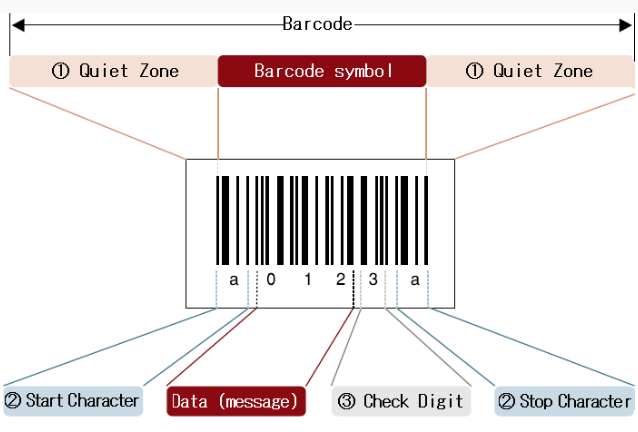
\includegraphics{barcodeComponents} \cite{barcode_componentsDiagram}

A quiet zone is blank margin located at both ends of the barcode. The minimum margin space is 2.5 mm. The quiet zone adds a constant reflection at either end of the barcode, allowing the scanner to clearly identify the start \& end of a barcode. If the width of a quiet zone is insufficient, barcodes can be hard for a scanner to read. 
\\~\\
The start character \& the stop character are characters (given in barcode form) representing the start \& the end of the data, respectively. The characters differ depending on the type of barcode.
\\~\\
The check digit is a numeral (given in barcode form) given just before the stop character. It helps the scanner verify whether the scanning was done correctly. The check digit is calculated as follows:

\begin{enumerate}
	\item Add the digits in the odd-numbered positions (positions 1, 3, 5...)
	\item Multiply the above by 3
	\item Add the digits in the even-numbered positions (positions 2, 4, 6...)
	\item Add results of steps 2 \& 3 together
	\item Find the closest multiple of 10 greater than the result of step 4
	\item Subtract the result of step 4 from the result of step 5
\end{enumerate}

Result 6 is the check digit. Now, to simplify the last two steps, let $c$ be the result obtained at step 4, and et $k$ be the smallest number such that $10k \geq c$. Now note that steps 5 and 6 state that you must perform $10k - c$. But by definition of $k$, we know that $10k - c \leq 10$
\[\implies 10k - c = (10k-c) \bmod 10 = 10 - c \bmod 10\]
We will use this result to create a function to calculate the check digit of a barcode...

\section{Simple barcode check digit calculator}
\include*{codes/tex/barcodeCheckDigit}

\chapter{Coding \& decoding}
\section{Definition \& purpose}
Letter coding is a mapping wherein alphabets of a string are converted into another alphabet using a specific rule. More precisely, letter coding is a mapping from the set of alphabets to the set of alphabets.
\\~\\
Number coding is a mapping wherein units of a string (unit can be decided by the coder, ex. words, alphabets, fixed size slices) are converted into a number using a specific rule. More precisely, letter coding is a mapping from the set of string units to the set of integers. We have witnessed number coding in this document in the chapter on cryptography, in the demonstration of RSA, where message partitions are first converted to integers (check document subsection \ref{rsaDemo}).
\\~\\
Coding in general is a mapping between units of two data representations (which may be same (as in letter coding) or different (as in number coding)). Note that for it to be possible to obtain the original data from coded data, there must be one-to-one mapping from the domain to the range of the coding map.
\\~\\
Some applications of coding:
\begin{itemize}
	\item Cryptography (messages are made secret using encryption \& decryption keys)
	\item Data compression (longer data is mapped to a more compact representation)
	\item Line coding (converting data into signals to be transmitted across distances)
\end{itemize}

\section{Caesar cipher}
This is the simplest letter coding rule. Here, given a definite order of alphabets (ex. 'a', 'b', 'c', 'd', ...), every alphabet $\alpha$ is mapped to the alphabet present at a fixed offset from the position of $\alpha$. Note that the ordered sequence of alphabets is circular, so if the offset position exceeds the length of the sequence, the coding process loops back to the first position \& continues accordingly.

\subsection{Python implementation}
For our implementation of Caesar cipher in Python, we make the following considerations
\begin{itemize}
	\item We are dealing with ASCII values, so $"z" = 122$, $"Z" = 90$
	\item If character is uppercase, choose $"Z"$ as the last alphabet
	\item If character is lowercase, choose $"z"$ as the last alphabet
\end{itemize}

\subsubsection{Assumptions, definitions \& notations}
Our very first assumption in this implementation is that the message to be coded is in regular English, with special characters or alphabets not being considered as part of the alphabet. Note that Caesar cipher can be designed to suit different languages \& use cases.
\\~\\
Note that we assume that the offset, which we shall denote as $k$, is such that $k \in Z_+, k < n$ (assuming we have $n$ possible letters), since due to the circular nature of Caesar cipher, any offset $k \geq n$ can be converted into a functionally identical offset $k \in Z_+, k < n$ using modulo $n$ i.e. doing $k_{new}=k_{old} \bmod n$.
\\~\\
Note that due to the very definition of Caesar cipher, we map the letters to be coded \& decoded to a fixed set of numerical indices (i.e. natural numbers separated by 1). For example, in regular English alphabets, we may give "a" = 1, "b = 2... "z" = 26. The ASCII values of English alphabets also form a mapping between letters \& a fixed set of indices, if we consider uppercase \& lowercase alphabets separately. The ASCII values of alphabets are what we will be using in our Python implementation. Non-English alphabets will remain untouched in our algorithm.
\\~\\
Consider a set of alphabets that are mapped to a fixed set of indices (ASCII values). Define $\alpha$ as the function that returns the index (ASCII value) of an alphabet. Denote any alphabet in the string as $c$, denote as $d$ as the Caesar cipher of $c$, \& denote $k \in Z_+$ as the offset. For simplicity of explanation, let $c$ be lowercase. Note that the same logic will apply for uppercase too.

\subsection{Encoding implementation}
Here, we will aim to obtain $\alpha(d)$ (i.e. the cipher alphabet) in terms of $\alpha(c)$ (i.e. the original alphabet). Now note that, assuming $c$ is a proper alphabet, we have that $\alpha("a") \leq \alpha(c) \leq \alpha("z")$.

\subsubsection{CASE 1: $\alpha(c)+k \leq \alpha("z")$}
\begin{equation} \label{caesarCipherEncodingEq1} \implies \alpha(d) = \alpha(c)+k \end{equation}

\subsubsection{CASE 2: $\alpha(c)+k > \alpha("z")$}
\begin{equation} \label{caesarCipherEncodingEq2} \implies \alpha(d) = (\alpha(c)+k) - \alpha(z) + \alpha("a") - 1 \end{equation}

\textbf{Explanation of the above logic}...\\
The logic for case 1 is trivial, based on the definition of Caesar cipher. To see why the logic for the case 2 holds, consider the following. To obtain the Caesar cipher, we may begin by simply adding the offset to the index of $c$, as in
\[\alpha(c)+k\]
But in case 2, $\alpha(c)+k > \alpha("z")$, which means $\alpha(c)+k$ is not the required cipher. Instead, we will count the number of digits exceeding $z$ i.e. $(\alpha(c)+k)-\alpha("z")$, \& obtain the alphabet that has this offset from $"z"$, considering that $"z"$ is looped back to $"a"$. This process can be computationally expressed as equation \ref{caesarCipherEncodingEq2}.

\include*{codes/tex/caesarCipherEncoding}

\subsection{Decoding implementation}
Here, we will aim to obtain $\alpha(c)$ (i.e. the original character) in terms of $\alpha(d)$. This also means that to be able to implement the decoding formula knowing only $d$, we must obtain the equivalent conditions of cases 1 \& 2 in terms of $\alpha(d)$. Now note that, assuming $d$ is a proper Caesar cipher of $c$, we have that $\alpha("a") \leq \alpha(d) \leq \alpha("z")$.
\subsubsection{CASE 1: $\alpha(c)+k \leq \alpha("z")$}
Hence, from the encoding implementation for this case i.e. equation \ref{caesarCipherEncodingEq1}, we get

\[\alpha(d) = \alpha(c)+k\]
\begin{equation} \label{caesarCipherDecodingEq1} \implies \alpha(c) = \alpha(d) - k \end{equation}
\\~\\
\textbf{Case 1 condition in terms of $\alpha(d)$}...\\
Now, note that by its very nature, $\alpha("a") \leq \alpha(c) \leq \alpha("z")$\\
$\implies \alpha("a") \leq \alpha(d) - k  \leq \alpha("z")$\\
Since $\alpha("a") \leq \alpha(d) \leq \alpha("z")$, the above condition, simply becomes\\
$\alpha("a") \leq \alpha(d) - k$\\
since $\alpha(d) - k < \alpha(d) \leq \alpha("z")$. Hence, $\alpha(d) - k$ needs to satisfy the above condition for the above decoding to take place.

\subsubsection{CASE 2: $\alpha(c)+k > \alpha("z")$}
Hence, from the encoding implementation for this case i.e. equation \ref{caesarCipherEncodingEq2}, we get
\[\alpha(d) = (\alpha(c)+k - \alpha("z") + \alpha("a") - 1\]
\begin{equation} \implies \alpha(c) = \alpha(d) - \alpha("a") + 1 - k + \alpha("z") \end{equation}
\\~\\
\textbf{Case 2 condition in terms of $\alpha(d)$}...\\
Now, note that the condition of case 2 is mutually exclusive from the condition of case 1 i.e. if condition of case 2 is true, condition of case 1 cannot be true. Now, from case 1, we got the equivalent condition in terms of $\alpha(d)$ as\\
$\alpha("a") \leq \alpha(d) - k$\\
Hence, this condition must be mutually exclusive from the equivalent condition of case 2 in terms of $\alpha(d)$. Hence, the condition of case 2 in terms of $\alpha(d)$ must be\\
$\alpha("a") > \alpha(d) - k$\\
Hence, $\alpha(d) - k$ needs to satisfy the above condition for the above decoding to take place. In any case, in the Python implementation, a mutually exclusive condition can be obtained by simply using "else".

\include*{codes/tex/caesarCipherDecoding}

\section{Randomised or arbitrary one-to-one coding}
Here, a symbol is mapped to another symbol without using a generalised rule, such that the mapping is one-to-one. Hence, the to code \& decode using this method, we need to define \& refer to a specified mapping table. However, when it comes to coding a natural language (ex. English), decoding can be done by analysing the frequencies of the symbols in the message. This works, because many languages tend to use certain letters more than others, in general. For example, in English, the most commonly used letter is 'e', followed by 't'. Given below is a relative usage frequency distribution of the occurrence of alphabets in the words listed in the main entries of the Concise Oxford Dictionary  (9th edition, 1995) \textit{(relative frequency of letter means the the proportion of the usage of the letter, rather than the total count)}.

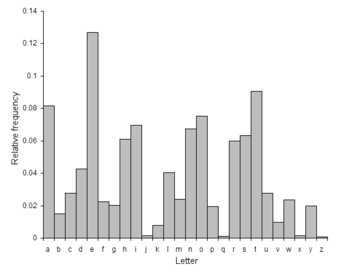
\includegraphics{englishLetterFrequencies} \cite{englishLetterFreqGraph}

Using such information about a language's usage, \& knowing the source language of a cipher, an arbitrary one-to-one coding can be cracked relatively easily.

\nocite{*}
\bibliographystyle{plain}
\bibliography{references}
\end{document}